\subsection{Attractive}
It is important that the information is attractive, eye-catching, with spark. Not only from a conceptual point of view
or functional as we saw in the relevant section, where we made clear the implication of the data and the importance
of its correct presentation, with a structure that guides the user in a logical and orderly manner.

It has to grab our attention, for this we can propose the following requirements, that is fun, entertaining,
modern, current, close, quality, beautiful and harmonious.

Although these characteristics are subjective, there are techniques to achieve these objectives.

Other more technical characteristics are: \\
textbf {Consistency.} Controls that perform the same actions must maintain the same design. The functionalities
they should also follow this principle \\

\textbf{Cleaning.} An ordered design will convey a better feeling and the user will be able to locate what they are looking for
more easily\\

\textbf{Simplicity.} The objective is to represent the information, we will flee from any unnecessary decoration that will embroil
the main objective. Remember that less is more. A complicated design, with many colors and different abstract shapes
it will be more difficult to interpret by the user \\


\textbf{Standards.} In the market there are several standards to which the user is accustomed and knows what to expect.
For example a magnifying glass, we relate it to the action of searching, if we use this icon, the user will quickly know that
function performs, however, if we use a completely new one, it can even confuse the user \\

\textbf{Familiarity.} The user will find it easier to manipulate or navigate the platform if he feels that
He is familiar and does not feel lost. For example, if we have an icon to choose a date, it would be highly recommended
use a calendar, although it is not a standard, we are used to recognize it \\

\textbf{Details.} A label with different typology or other color may disturb the user's perception. If not
we want to highlight something in particular, it seems like an error \\

\textbf{Sena de identidad.} It is highly recommended to use something unique that identifies us and that the user is capable of
to recognize ourselves quickly, this can be an image, a combination of colors, a logo, etc.
\subsubsection{How to solve it} 
To be able to make an attractive design, it is necessary to study the trends of the moment, the good practices of design and apply them.
It is highly recommended to maintain a simple and clean design, use standards or mechanisms that are familiar to users,
take care of the details and mark our identity.

\subsubsection{How we solve it. Aire Guru} 


As we commented previously the design has been based on material design, use straight lines, difference
different sections by rectangles and uses colors that constrain enough between the information and the background.
The background color for the graphics is white, since most use different colors and white is a color
neutral. Only the shades of blue, gray and white are used. In addition, a font that is easy to read if decoration is used.

The sections are arranged neatly and structured. These are composed of a header and a body.

The central page consists of a header, the body and a footer. Both the header and the footer are static,
they are shown in all the pages and they continue all the information available to navigate between pages.
The body is divided into three horizontal sections, the upper zone with the map and the general information of the selected point,
the average zone where we can filter the polluting agents by medical conditions and information about the current situation and the
lower area where we will find the zone and custom history.

\begin{figure}[ht]
    \centering
    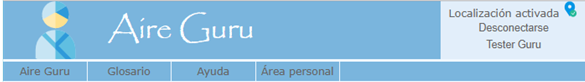
\includegraphics[width=12cm]{heading}
    \caption{Heading}
\end{figure}
The standard components are:
\begin{itemize}
\item the buttons, which darken when they are selected and use a more result key when they are selected.
\item Pestanas, with a similar behavior and a standard pestana aspect
\item Waiting symbol, rotating circle
\item Links, underlined texts
\item Search bar, like the one we find in search engines
\end{itemize}

\begin{figure}[ht]
    \centering
   \subfigure[Searching bar]
    {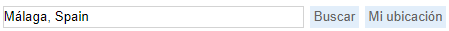
\includegraphics[width=5.5cm  ]{searchingBar}}
    \hfill
    \subfigure [Tabs]
       { 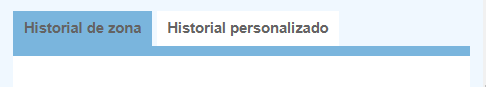
\includegraphics[width=5.5cm]{tabs}}
    \vfill
     \subfigure[Link]
     { \centering 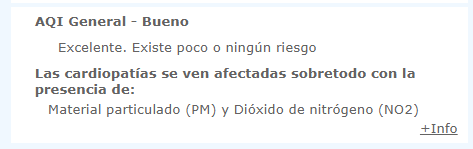
\includegraphics[width=6cm]{link}}
  
  \caption{Filters}
    \end{figure}
    The elements that give us familiarity are the iconography that we use to show the AQI. We use clouds, by representation
    of the air, the environment, it is accompanied by a heart if the quality is good, of a symbol of exclamation if it is poor, of a cross if it is
    bad and we change to a gas mask if the state is unhealthy.
    
    Today we are all used to GoogleMaps maps, so it has been integrated to represent the map and not another,
    since users are familiar with how they look and how they are used.
    
    The symbol of our tool is a genius, that is to say a guru, besides, we include "Air" in the logo, because it represents perfectly
    what we show Our tool is the genius of Air.
    
    Finally, it has been taken into account that the user can use our tool in different devices, so they have been implemented
    two different formats, one for larger screens such as the computer and another for smaller format for tablet or mobile.
\elsparagraph{Evaluation}  
\begin{itemize}
    \done
    \crossed Although there have been attempts to implement the design lines that are now on the market, the design can be improved
    
\end{itemize}
\newpage